\emph{Qt} jest międzyplatformowym (ang. cross-platform) frameworkiem aplikacyjnym, najczęściej używany w tworzeniu oprogramowania z graficznym interfejsem użytkownika.
Dodatkowo biblioteka zawiera moduły wspomagające między innymi:
\begin{itemize}
\item międzyplatformowe \emph{API}\footnote{ang. Application Programming Interface} dostępu do systemu plików,
\item dostęp do relacyjnych baz danych,
\item manipulacja XML,
\item międzyplatformowe zarządzanie wątkami,
\item międzyplatformowe wsparcie dla sieci.
\end{itemize}

Aplikacje \emph{Qt} tworzone są w języku C++ rozszerzonym o dodatkowe słowa kluczowe i makra, których obsługą zajmuje się program moc (Meta-Object Compiler). Największym uzupełnieniem wniesionym do języka przez framework jest system sygnałów i slotów.

\emph{Qt} wspiera największe platformy takie jak:
\begin{itemize}
\item Windows,
\item Windows CE,
\item Symbian,
\item OS X,
\item X11 (Linux, FreeBSD, Solaris, AIX i inne),
\item Maemo, MeeGo.
\end{itemize}

Framework w wersji 5, która jest akutalnie w fazie beta, ma być dostępny również na wszystkie popularne platformy mobilne takie jak Android, iOS i Windows 8.

W tym podrozdziale zostaną przedstawione mechanizmy biblioteki \emph{Qt} wykorzystane przy tworzeniu projektu, o którym stanowi niniejsza praca. 

\subsection{System zdarzeń}
W \emph{Qt} zdarzenia są obiektami dziedziczącymi po klasie \emph{QEvent}, reprezentującymi zajście pewnego zjawiska wewnątrz aplikacji lub będącymi wynikiem oddziaływania z zewnątrz, o którym aplikacja powinna wiedzieć. Zdarzenia mogą być przetworzone przez wszystkie obiekty dziedziczące po klasie \emph{QObject}, która dostarcza podstawowej struktury i logiki niezbędnej do ich obsługi. 

Kiedy system operacyjny generuje sygnał o zajściu pewnego zdarzenia, \emph{Qt} dokonuje jego konwersji na odpowiedni i platformowo niezależny format. Każde zdarzenie jest następnie przekazywane do \emph{kolejki zdarzeń} odpowiedniego wątku. Kolejka przechowuje i w odpowiednim momencie rozdysponowywuje zdarzenia do odpowiadających im obiektów odbiorców poprzez wywołanie metody \emph{QObject::event()} wewnątrz której następuje decyzja dotycząca dalszego przetwarzania, zależna od rodzaju zdarzenia. 

Niektóre zdarzenia, takie jak na przykład \emph{QMouseEvent} czy \emph{QKeyEvent} pochodzą bezpośrednio od systemu operacyjnego. Inne, jak na przykład \emph{QTimerEvent} czy \emph{QPaintEvent} pochodzą z innych źródeł, nierzadko z wnętrza samej aplikacji (np. do komunikacji między wątkami). Warto w tym miejscu zaznaczyć, że rysowanie w \emph{Qt} nie jest operacją wywoływaną przez system operacyjny lecz przez samą aplikację oraz rysowanie z wnętrza obsługi zdarzenia \emph{QPaintEvent} jest jedynym sposobem na renderowanie graficznego interfejsu aplikacji. Pociąga to za sobą pewne problemy opisane w dalszej części pracy.

\subsection{System widgetów}
Widget'em w bibliotece \emph{Qt} nazywamy obiekt reprezentujący elementy graficznego interfejsu użytkownika takie jak przyciski, listy rozwijane, menu, okna i inne. Klasa \emph{QWidget}\cite{qwidget} jest typem bazowym dla wszystkich widgetów i udostępnia niezbędne metody dotyczące renderowania oraz obsługi zdarzeń dzięki czemu w łatwy sposób można uzyskać dostęp do całego interfejsu aplikacji.

Interfejs użytkownika w aplikacjach opartych o framework \emph{Qt} tworzy strukturę hierarchiczną powiązanych ze sobą obiektów klasy QWidget. Wykorzystując ten fakt w łatwy sposób można odtworzyć tą strukturę w innych technologiach, np. tworząc identyczną strukturę w języku HTML. Fakt ten został wykorzystany w niniejszej pracy.

\subsection{System rysowania}
\label{system_rysowania}
Rysowanie w bibliotece \emph{Qt} standardowo zostało zaimplementowane dla rysowania na ekranie oraz urządzeniach drukujących wykorzystując natywne \emph{API} systemu operacyjnego, dla którego dana wersja \emph{Qt} została skompilowana. Moduł ten jest niejako opakowaniem dla wywołań systemowych, ujednolicając jego logikę i umożliwiając pełną przenośność aplikacji. Na rysunku \ref{paintsystem-core} przedstawiony został kaskadowy model systemu rysowania w \emph{Qt}. Jest to \emph{model trójwarstwowy} i każda z klas ma swoje określone zadanie w całym procesie renderowania. Główną zaletą takiego podejścia jest ujednolicenie przepływu procesu rysowania dla różnych urządzeń wyjściowych oraz umożliwienie łatwego sposobu dla dodawania nowych funkcjonalności.

Klasa \emph{QPainter} udostępnia jednolity interfejs umożliwjający wykonywanie operacji rysowania różnych obiektów takich jak linie, okręgi, prostokąty, obrazy oraz umożliwia zastosowanie różnego rodzaju przekształceń, styli czy transformacji macierzowych. 

Klasa \emph{QPaintDevice} stanowi abstrakcję dla dwuwymiarowej przestrzeni na której obiekty klasy \emph{QPainter} mogą wykonywać operacje rysowania. Udostępnia ona różnego rodzaju informacje dotyczące specyfiki urządzenia wyjściowego, które mogą być wykorzystane np. do optymalizacji procesu rysowania. 

Klasa \emph{QPaintEngine} udostępnia interfejs, za pomocą którego obiekty klasy \emph{QPainter} będą mogły wykonywać operacje rysowania na różnego rodzaju urządzeniach wyjściowych. Klasa \emph{QPaintEngine} jest używana wewnątrz klas \emph{QPainter} oraz \emph{QPaintDevice} i jest ukryta przed aplikacjiami dopóki programista nie zechce stworzyć obsługi dla nowego rodzaju urządzenia wyjściowego. W niniejszej pracy taki właśnie scenariusz został wykorzystany.
 
// TODO: Obrazek w formie wektorowej

\begin{figure}[!h]
  \centering
  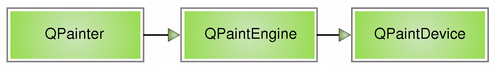
\includegraphics[width=\textwidth,height=!]{img/paintsystem-core.png}
  \caption{Schemat budowy systemu renderowania w bibliotece \emph{Qt}}
  \label{paintsystem-core}
\end{figure}